% Generated by pysimcount.pfboundchilds -- do not edit; regenerate instead.
% figure: bound-min-cnot-all-formulas -- Every formula, X-Y-Z grouping, CNOT vs n, r from the minimised norm bound
% r from minimised norm bound (Childs et al. 2018, Def. 2; extended to every formula); bound settings {"kind": "min", "budget": "count", "constant": "childs"}
% NumPy seeds [1, 2, 3, 4, 5, 6, 7, 8, 9, 10]; t = n; sizes [4, 5, 6, 7, 8, 9, 10, 11, 13, 20, 30, 50, 70, 100, 200, 300, 500]; cz: eps_trotter = 0.001, merged, simcount template
% CNOT = exact affine per-step count x r; affine model checked against 880 run rows (n = 4-11)
% pruning: up to 3 removed, never one of the 2 cheapest at any n
% shown: suzuki2, suzuki4, mo-q6, mo-q14, bm-q10, mo-o8-q21, morales-y8m10, morales-m8
% removed: lie-trotter, suzuki6, suzuki8
% figure made at git_commit=eed0c490bd2a7ed3c821acf76ae930c79d2195f6 git_dirty=True
% WARNING: made from uncommitted code; the commit above does not reproduce it.
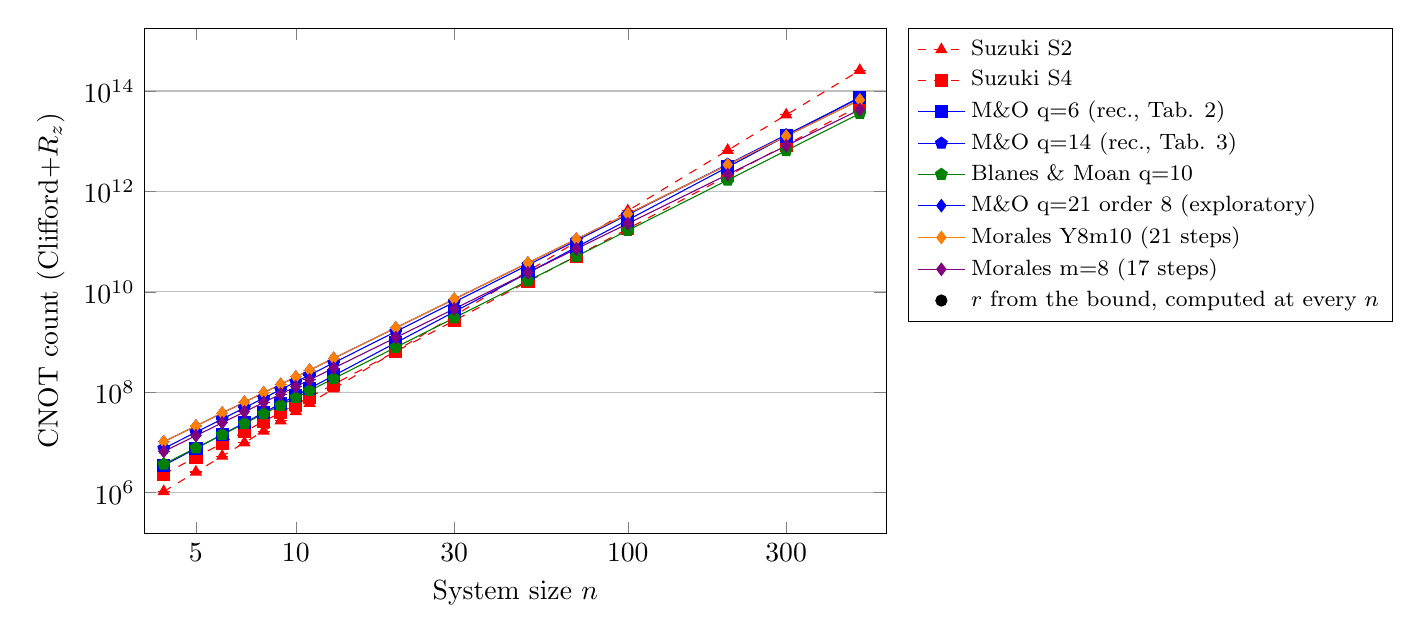
\begin{tikzpicture}
  \begin{loglogaxis}[
    width=11cm, height=8cm,
    xlabel={System size $n$},
    ylabel={CNOT count (Clifford+$R_z$)},
    xtick={5,10,30,100,300}, xticklabels={5,10,30,100,300},
    xmin=3.5, xmax=600,
    ymajorgrids=true,
    legend pos=outer north east,
    legend cell align=left,
    legend style={font=\footnotesize},
  ]
    % suzuki2: r from the bound at every n; point = mean over seeds, bars min..max over seeds
    \addplot[red, dashed, mark=triangle*, mark size=2.2pt, mark options={solid, fill=red}, error bars/.cd, y dir=both, y explicit, error bar style={solid}] coordinates {
      (4,1.06016e+06) += (0,0) -= (0,0)
      (5,2.587e+06) += (0,0) -= (0,0)
      (6,5.36268e+06) += (0,0) -= (0,0)
      (7,9.93272e+06) += (0,0) -= (0,0)
      (8,1.69418e+07) += (0,0) -= (0,0)
      (9,2.71339e+07) += (0,0) -= (0,0)
      (10,4.13519e+07) += (0,0) -= (0,0)
      (11,6.0538e+07) += (0,0) -= (0,0)
      (13,1.18079e+08) += (0,0) -= (0,0)
      (20,6.61309e+08) += (0,0) -= (0,0)
      (30,3.34734e+09) += (0,0) -= (0,0)
      (50,2.58249e+10) += (0,0) -= (0,0)
      (70,9.92034e+10) += (0,0) -= (0,0)
      (100,4.13158e+11) += (0,0) -= (0,0)
      (200,6.61021e+12) += (0,0) -= (0,0)
      (300,3.34637e+13) += (0,0) -= (0,0)
      (500,2.58204e+14) += (0,0) -= (0,0)
    };
    \addlegendentry{Suzuki S2}
    % suzuki4: r from the bound at every n; point = mean over seeds, bars min..max over seeds
    \addplot[red, dashed, mark=square*, mark size=2.2pt, mark options={solid, fill=red}, error bars/.cd, y dir=both, y explicit, error bar style={solid}] coordinates {
      (4,2.33755e+06) += (0,0) -= (0,0)
      (5,5.09817e+06) += (0,0) -= (0,0)
      (6,9.64202e+06) += (0,0) -= (0,0)
      (7,1.65263e+07) += (0,0) -= (0,0)
      (8,2.63575e+07) += (0,0) -= (0,0)
      (9,3.97868e+07) += (0,0) -= (0,0)
      (10,5.75064e+07) += (0,0) -= (0,0)
      (11,8.02499e+07) += (0,0) -= (0,0)
      (13,1.43923e+08) += (0,0) -= (0,0)
      (20,6.49228e+08) += (0,0) -= (0,0)
      (30,2.68105e+09) += (0,0) -= (0,0)
      (50,1.6009e+10) += (0,0) -= (0,0)
      (70,5.19507e+10) += (0,0) -= (0,0)
      (100,1.80947e+11) += (0,0) -= (0,0)
      (200,2.0458e+12) += (0,0) -= (0,0)
      (300,8.45378e+12) += (0,0) -= (0,0)
      (500,5.05115e+13) += (0,0) -= (0,0)
    };
    \addlegendentry{Suzuki S4}
    % mo-q6: r from the bound at every n; point = mean over seeds, bars min..max over seeds
    \addplot[blue, solid, mark=square*, mark size=2.2pt, mark options={solid, fill=blue}, error bars/.cd, y dir=both, y explicit, error bar style={solid}] coordinates {
      (4,3.4934e+06) += (0,0) -= (0,0)
      (5,7.61925e+06) += (0,0) -= (0,0)
      (6,1.44105e+07) += (0,0) -= (0,0)
      (7,2.47006e+07) += (0,0) -= (0,0)
      (8,3.93952e+07) += (0,0) -= (0,0)
      (9,5.94684e+07) += (0,0) -= (0,0)
      (10,8.59555e+07) += (0,0) -= (0,0)
      (11,1.19952e+08) += (0,0) -= (0,0)
      (13,2.15132e+08) += (0,0) -= (0,0)
      (20,9.70498e+08) += (0,0) -= (0,0)
      (30,4.00794e+09) += (0,0) -= (0,0)
      (50,2.3933e+10) += (0,0) -= (0,0)
      (70,7.76668e+10) += (0,0) -= (0,0)
      (100,2.70523e+11) += (0,0) -= (0,0)
      (200,3.05864e+12) += (0,0) -= (0,0)
      (300,1.26393e+13) += (0,0) -= (0,0)
      (500,7.5521e+13) += (0,0) -= (0,0)
    };
    \addlegendentry{M\&O q=6 (rec., Tab. 2)}
    % mo-q14: r from the bound at every n; point = mean over seeds, bars min..max over seeds
    \addplot[blue, solid, mark=pentagon*, mark size=2.2pt, mark options={solid, fill=blue}, error bars/.cd, y dir=both, y explicit, error bar style={solid}] coordinates {
      (4,7.63435e+06) += (0,0) -= (0,0)
      (5,1.60415e+07) += (0,0) -= (0,0)
      (6,2.94284e+07) += (0,0) -= (0,0)
      (7,4.91568e+07) += (0,0) -= (0,0)
      (8,7.66682e+07) += (0,0) -= (0,0)
      (9,1.13471e+08) += (0,0) -= (0,0)
      (10,1.61142e+08) += (0,0) -= (0,0)
      (11,2.21313e+08) += (0,0) -= (0,0)
      (13,3.85962e+08) += (0,0) -= (0,0)
      (20,1.61983e+09) += (0,0) -= (0,0)
      (30,6.24984e+09) += (0,0) -= (0,0)
      (50,3.42566e+10) += (0,0) -= (0,0)
      (70,1.05071e+11) += (0,0) -= (0,0)
      (100,3.44736e+11) += (0,0) -= (0,0)
      (200,3.47032e+12) += (0,0) -= (0,0)
      (300,1.3399e+13) += (0,0) -= (0,0)
      (500,7.34983e+13) += (0,0) -= (0,0)
    };
    \addlegendentry{M\&O q=14 (rec., Tab. 3)}
    % bm-q10: r from the bound at every n; point = mean over seeds, bars min..max over seeds
    \addplot[green!50!black, solid, mark=pentagon*, mark size=2.2pt, mark options={solid, fill=green!50!black}, error bars/.cd, y dir=both, y explicit, error bar style={solid}] coordinates {
      (4,3.7123e+06) += (0,0) -= (0,0)
      (5,7.79984e+06) += (0,0) -= (0,0)
      (6,1.43079e+07) += (0,0) -= (0,0)
      (7,2.38991e+07) += (0,0) -= (0,0)
      (8,3.72726e+07) += (0,0) -= (0,0)
      (9,5.51633e+07) += (0,0) -= (0,0)
      (10,7.83362e+07) += (0,0) -= (0,0)
      (11,1.07585e+08) += (0,0) -= (0,0)
      (13,1.87617e+08) += (0,0) -= (0,0)
      (20,7.87331e+08) += (0,0) -= (0,0)
      (30,3.03755e+09) += (0,0) -= (0,0)
      (50,1.66481e+10) += (0,0) -= (0,0)
      (70,5.10601e+10) += (0,0) -= (0,0)
      (100,1.6752e+11) += (0,0) -= (0,0)
      (200,1.68623e+12) += (0,0) -= (0,0)
      (300,6.51037e+12) += (0,0) -= (0,0)
      (500,3.57103e+13) += (0,0) -= (0,0)
    };
    \addlegendentry{Blanes \& Moan q=10}
    % mo-o8-q21: r from the bound at every n; point = mean over seeds, bars min..max over seeds
    \addplot[blue, solid, mark=diamond*, mark size=2.2pt, mark options={solid, fill=blue}, error bars/.cd, y dir=both, y explicit, error bar style={solid}] coordinates {
      (4,1.03646e+07) += (0,0) -= (0,0)
      (5,2.138e+07) += (0,0) -= (0,0)
      (6,3.86325e+07) += (0,0) -= (0,0)
      (7,6.3709e+07) += (0,0) -= (0,0)
      (8,9.82668e+07) += (0,0) -= (0,0)
      (9,1.44019e+08) += (0,0) -= (0,0)
      (10,2.02737e+08) += (0,0) -= (0,0)
      (11,2.76236e+08) += (0,0) -= (0,0)
      (13,4.75081e+08) += (0,0) -= (0,0)
      (20,1.92344e+09) += (0,0) -= (0,0)
      (30,7.174e+09) += (0,0) -= (0,0)
      (50,3.76772e+10) += (0,0) -= (0,0)
      (70,1.12353e+11) += (0,0) -= (0,0)
      (100,3.57779e+11) += (0,0) -= (0,0)
      (200,3.39843e+12) += (0,0) -= (0,0)
      (300,1.26831e+13) += (0,0) -= (0,0)
      (500,6.66564e+13) += (0,0) -= (0,0)
    };
    \addlegendentry{M\&O q=21 order 8 (exploratory)}
    % morales-y8m10: r from the bound at every n; point = mean over seeds, bars min..max over seeds
    \addplot[orange, solid, mark=diamond*, mark size=2.2pt, mark options={solid, fill=orange}, error bars/.cd, y dir=both, y explicit, error bar style={solid}] coordinates {
      (4,1.03646e+07) += (0,0) -= (0,0)
      (5,2.138e+07) += (0,0) -= (0,0)
      (6,3.86325e+07) += (0,0) -= (0,0)
      (7,6.3709e+07) += (0,0) -= (0,0)
      (8,9.82668e+07) += (0,0) -= (0,0)
      (9,1.44019e+08) += (0,0) -= (0,0)
      (10,2.02737e+08) += (0,0) -= (0,0)
      (11,2.76236e+08) += (0,0) -= (0,0)
      (13,4.75081e+08) += (0,0) -= (0,0)
      (20,1.92344e+09) += (0,0) -= (0,0)
      (30,7.174e+09) += (0,0) -= (0,0)
      (50,3.76772e+10) += (0,0) -= (0,0)
      (70,1.12353e+11) += (0,0) -= (0,0)
      (100,3.57779e+11) += (0,0) -= (0,0)
      (200,3.39843e+12) += (0,0) -= (0,0)
      (300,1.26831e+13) += (0,0) -= (0,0)
      (500,6.66564e+13) += (0,0) -= (0,0)
    };
    \addlegendentry{Morales Y8m10 (21 steps)}
    % morales-m8: r from the bound at every n; point = mean over seeds, bars min..max over seeds
    \addplot[violet, solid, mark=diamond*, mark size=2.2pt, mark options={solid, fill=violet}, error bars/.cd, y dir=both, y explicit, error bar style={solid}] coordinates {
      (4,6.6378e+06) += (0,0) -= (0,0)
      (5,1.3691e+07) += (0,0) -= (0,0)
      (6,2.47382e+07) += (0,0) -= (0,0)
      (7,4.07951e+07) += (0,0) -= (0,0)
      (8,6.29225e+07) += (0,0) -= (0,0)
      (9,9.22185e+07) += (0,0) -= (0,0)
      (10,1.29814e+08) += (0,0) -= (0,0)
      (11,1.76874e+08) += (0,0) -= (0,0)
      (13,3.04191e+08) += (0,0) -= (0,0)
      (20,1.23151e+09) += (0,0) -= (0,0)
      (30,4.59308e+09) += (0,0) -= (0,0)
      (50,2.41214e+10) += (0,0) -= (0,0)
      (70,7.19279e+10) += (0,0) -= (0,0)
      (100,2.29044e+11) += (0,0) -= (0,0)
      (200,2.17553e+12) += (0,0) -= (0,0)
      (300,8.119e+12) += (0,0) -= (0,0)
      (500,4.26685e+13) += (0,0) -= (0,0)
    };
    \addlegendentry{Morales m=8 (17 steps)}
    \addlegendimage{only marks, black, mark=*, mark options={solid, fill=black}}
    \addlegendentry{$r$ from the bound, computed at every $n$}
  \end{loglogaxis}
\end{tikzpicture}
